\documentclass[10pt]{article}
\usepackage{graphicx}
\usepackage[margin=1.5cm]{geometry}
\usepackage{amsmath}
\def\brcurs{{\mbox{$\resizebox{.16in}{.08in}{
\includegraphics{BoldR}}$}}}
\def\rcurs{{\mbox{$\resizebox{.16in}{.08in}{
\includegraphics{ScriptR}}$}}}

\begin{document}
\twocolumn

\title{Tuesday Warm-up: Motional emf and Faraday's Law}
\author{Prof. Jordan C. Hanson}

\maketitle

\begin{figure}
\centering
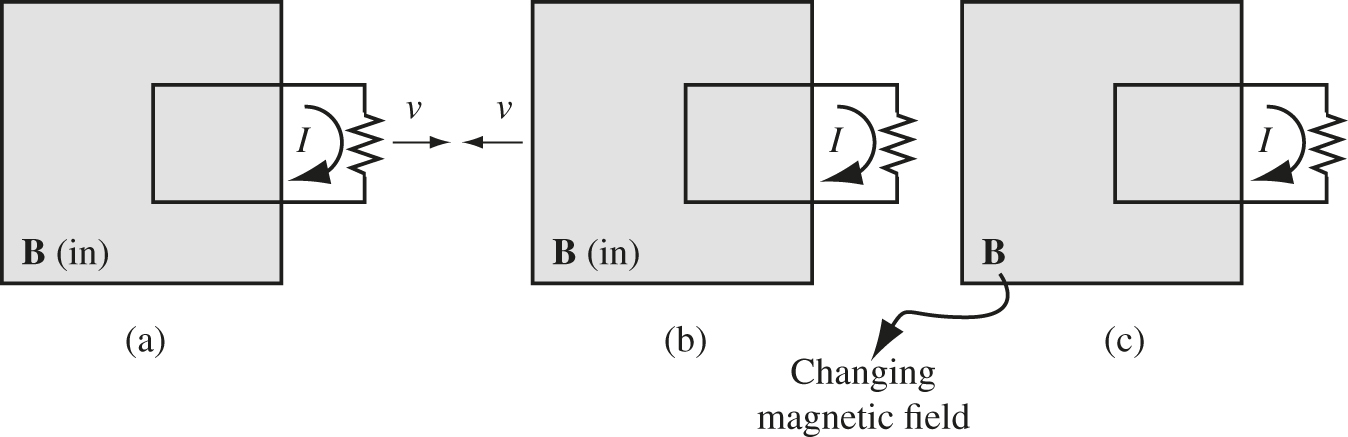
\includegraphics[width=0.42\textwidth]{figures/7_21.jpg}
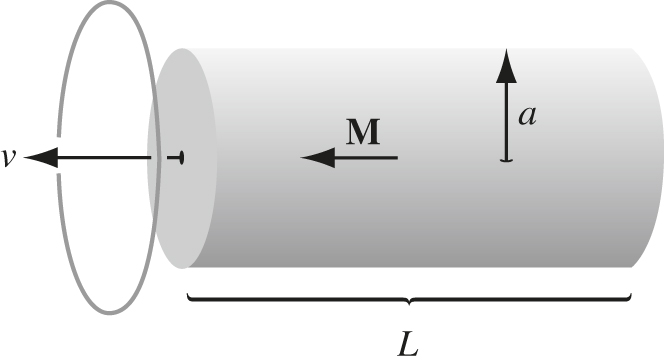
\includegraphics[width=0.23\textwidth]{figures/7_22.jpg} \hspace{0.33cm}
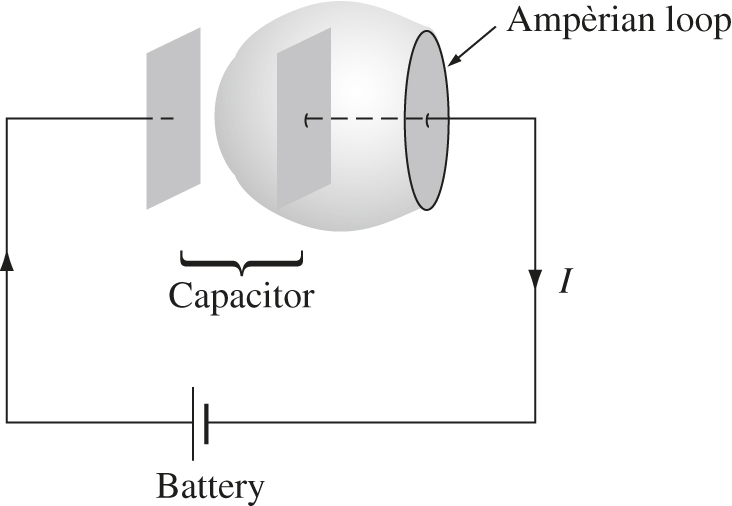
\includegraphics[width=0.23\textwidth]{figures/7_43.jpg}
\caption{\label{fig:1} (Top) Three tests of Faraday's Law. (Bottom left) A magnet passes through a loop of wire at constant velocity.  (Bottom right) An emf charges a capacitor.}
\end{figure}

\section{Memory Bank}

\begin{itemize}
\item \textbf{Definition of emf}:
\begin{equation}
\mathcal{E} = \oint \mathbf{E} \cdot d\mathbf{l}
\end{equation}
\item \textbf{Flux rule and emf}:
\begin{align}
\mathcal{E} &= -\frac{d\Phi}{dt} \\
\Phi &= \int \mathbf{B} \cdot d\mathbf{a}
\end{align}
\item \textbf{Faraday's Law}:
\begin{equation}
\nabla \times \mathbf{E} = -\frac{\partial \mathbf{B}}{\partial t}
\end{equation}
\end{itemize}

\section{Ohm's Law and Motional emf}

\begin{enumerate}
\item Consider Fig. \ref{fig:1} (top).  (a) Why is there an induced emf in the wire loop that moves to the left? (b) Why is there an induced emf in the wire loop if the $\mathbf{B}$-field moves to the right? (c) Why is there an induced emf if the strength of the field in the wire loop changes? \\ \vspace{3cm}
\item Consider Fig. \ref{fig:1} (bottom left).  A long cylindrical magnet of length $L$ and radius $a$ carries a uniform magnetization $\mathbf{M}$ parallel to its axis.  It passes at constant velocity $v$ through a circular wire ring of radius $b$.  Graph the induced emf as a function of time. \\ \vspace{3.5cm}
\end{enumerate}

\section{Faraday's Law}

\begin{enumerate}
\item Using the definition of emf and magnetic flux, construct a proof for the differential form of Faraday's law, via Stoke's Law. \\ \vspace{2cm}
\item Suppose two identical solenoids with turns per unit length $n$ and radius $a$ are arranged concentrically.  The following emf is connected to one solenoid:
\begin{equation}
\mathcal{E} = \mathcal{E}_0 \sin(2\pi f t)
\end{equation}
What is the emf induced in the other solenoid? \\ \vspace{2cm}
\item Turns out we need to fix Amp\`{e}re's Law.  Consider \ref{fig:1} (bottom right).  What is $I_{\rm enc}$ for the flat and curved surfaces?
\end{enumerate}

\end{document}
